\documentclass{beamer}

\usepackage{hyperref}
\usepackage{fancyhdr}
\usepackage{nameref}
\usepackage[symbol]{footmisc}
\usepackage{minitoc}
\usepackage{color}
\usepackage{amsmath}
\usepackage[francais]{babel}
\usepackage{natbib}
\usepackage{amssymb}
\usepackage[utf8]{inputenc}
\usepackage[footheight=1em]{beamerthemeboxes}
\usepackage{array}
\setcounter{tocdepth}{3}

\newcommand{\HRule}{\rule{\linewidth}{0.5mm}}
\renewcommand{\thefootnote}{\fnsymbol{footnote}}
\renewcommand{\contentsname}{Table des matières}

% Macros relatives à la traduction de PH avec arcs neutralisants vers PH à k-priorités fixes

% Macros générales
%\newcommand{\ie}{\textit{i.e.} }
\newcommand{\segm}[2]{\llbracket #1; #2 \rrbracket}
%\newcommand{\f}[1]{\mathsf{#1}}

% Notations générales pour PH
\newcommand{\PH}{\mathcal{PH}}
%\newcommand{\PHs}{\mathcal{S}}
\newcommand{\PHs}{\Sigma}
%\newcommand{\PHp}{\mathcal{P}}
\newcommand{\PHp}{\textcolor{red}{\mathcal{P}}}
%\newcommand{\PHproc}{\mathcal{P}}
\newcommand{\PHproc}{\mathbf{Proc}}
\newcommand{\Proc}{\PHproc}
\newcommand{\PHh}{\mathcal{H}}
\newcommand{\PHa}{\PHh}
%\newcommand{\PHa}{\mathcal{A}}
\newcommand{\PHl}{\mathcal{L}}
\newcommand{\PHn}{\mathcal{N}}
\newcommand{\PHt}{\mathcal{H}_{t}} % Ensemble des action du T-PH avec des actions temporisées

\newcommand{\PHhitter}{\mathsf{hitter}}
\newcommand{\PHtarget}{\mathsf{target}}
\newcommand{\PHbounce}{\mathsf{bounce}}
%\newcommand{\PHsort}{\Sigma}
\newcommand{\PHsort}{\PHs}
%State of PH
\newcommand{\PHst}{\zeta}

%Automata Network
\newcommand{\AN}{\mathcal{AAN}}
\newcommand{\TAN}{T-\mathcal{AN}}
\newcommand{\ANsort}{\Sigma}
\newcommand{\ANbound}[1]{\operatorname{b}(#1)}
\newcommand{\ANstate}{\mathcal{S}}
\newcommand{\ANtrans}{\mathcal{T}}
\newcommand{\ANst}{\zeta}
%\newcommand{\LS}{\textbf{LS}}
\newcommand{\LS}{\mathcal{LS}}
\newcommand{\ANgt}{\rightarrow}
\newcommand{\ANgtu}[1]{\ANgt_{#1}}
\newcommand{\origin}[1]{\mathsf{ori}(#1)}
\newcommand{\condition}[1]{\mathsf{cond}(#1)}
\newcommand{\destination}[1]{\mathsf{dest}(#1)}
%\newcommand{\ANuexp}[1]{U^{#1}}
\newcommand{\ANuexpsymbol}{\,\mathcal{U}}
\newcommand{\ANuexp}[1]{\ANuexpsymbol^{#1}}
\newcommand{\U}{\ANuexpsymbol}
\newcommand{\Ua}{\ANuexp{\mathsf{asyn}}}
\newcommand{\Us}{\ANuexp{\mathsf{syn}}}
\newcommand{\ANglobalstate}[1]{\langle #1 \rangle}
\newcommand{\ANltsymb}[4]{#1 \overset{#2}{#4} #3}
\newcommand{\ANlt}[3]{\ANltsymb{#1}{#2}{#3}{\rightarrow}}
\newcommand{\ANlts}[3]{\ANltsymb{#1}{\{#2\}}{#3}{\longrightarrow}}
\newcommand{\ANltsc}[3]{\textcolor{commentgray}{\ANlts{#1}{#2}{#3}}}
\newcommand{\aiellaj}{\ANlt{a_i}{\ell}{a_j}}
\newcommand{\trace}{\mathsf{trace}}
\newcommand{\successiverep}{\mathsf{sr}}

%\newcommand{\PHfrappeur}{\mathsf{frappeur}}
%\newcommand{\PHcible}{\mathsf{cible}}
%\newcommand{\PHbond}{\mathsf{bond}}
%\newcommand{\PHsorte}{\mathsf{sorte}}
%\newcommand{\PHbloquant}{\mathsf{bloquante}}
%\newcommand{\PHbloque}{\mathsf{bloquee}}

%\newcommand{\PHfrappeR}{\textcolor{red}{\rightarrow}}
%\newcommand{\PHmonte}{\textcolor{red}{\Rsh}}

\newcommand{\PHhitA}{\rightarrow}
\newcommand{\PHhitB}{\Rsh}
%\newcommand{\PHfrappe}[3]{\mbox{$#1\PHhitA#2\PHhitB#3$}}
%\newcommand{\PHfrappebond}[2]{\mbox{$#1\PHhitB#2$}}
\newcommand{\PHhit}[3]{#1\PHhitA#2\PHhitB#3}
\newcommand{\PHfrappe}{\PHhit}
\newcommand{\PHhbounce}[2]{#1\PHhitB#2}
\newcommand{\PHobj}[2]{\mbox{$#1\PHhitB^*\!#2$}}
\newcommand{\PHobjectif}{\PHobj}
\newcommand{\PHconcat}{::}
%\newcommand{\PHneutralise}{\rtimes}
\def\Sce{\mathbf{Sce}}

% Actions plurielles
\newcommand{\PHhitmultsymbol}{\rightarrowtail}
\newcommand{\PHhitmult}[2]{\mbox{$#1 \PHhitmultsymbol #2$}}
\newcommand{\PHfrappemult}{\PHhitmult}
\newcommand{\PHfrappemults}[2]{\PHhitmult{\{#1\}}{\{#2\}}}

%Action plurielle avec délai
\newcommand{\PHhitdelayB}{\Rsh}
\newcommand{\PHhitdelayA}[1]{\xrightarrow{#1} }
\newcommand{\PHhitdelay}[4]{#1\PHhitdelayA{#2} #3 \PHhitdelayB #4}
\newcommand{\PHfrappedelay}{\PHhitdelay}

\def\PHget#1#2{{#1[#2]}}
%\newcommand{\PHchange}[2]{#1\langle #2 \rangle}
%\newcommand{\PHchange}[2]{(#1 \Lleftarrow #2)}
%\newcommand{\PHarcn}[2]{\mbox{$#1\PHneutralise#2$}}
\newcommand{\PHplay}{\cdot}

\newcommand{\PHstate}[1]{\mbox{$\langle #1 \rangle$}}
\newcommand{\PHetat}{\PHstate}

\def\supp{\mathsf{support}}
\def\first{\mathsf{first}}
\def\last{\mathsf{last}}

\def\DNtrans{\rightarrow_{ADN}}
\def\DNdef{(\mathbb F, \langle f^1, \dots, f^n\rangle)}
\def\DNdep{\mathsf{dep}}
\def\PHPtrans{\rightarrow_{PH}}
\def\get#1#2{#1[{#2}]}
\def\encodeF#1{\mathbf{#1}}
\def\toPH{\encodeF{PH}}
\def\card#1{|#1|}
\def\decode#1{\llbracket#1\rrbracket}
\def\encode#1{\llparenthesis#1\rrparenthesis}
\def\Hits{\PHa}
\def\hit{\PHhit}
\def\play{\cdot}

\def\Pint{\textsc{PINT}}

\newcommand{\sN}{\mathbb{N}}

\input{macros/macros-ph}
\input{macros/tikzstyles2.tex}

\setbeamertemplate{footline}{
\leavevmode
\hbox{\hspace*{-0.06cm}
\begin{beamercolorbox}[wd=.2\paperwidth,ht=2.25ex,dp=1ex,center]{author in head/foot}
	\usebeamerfont{author in head/foot}\insertshortauthor  %~~(\insertshortinstitute)
\end{beamercolorbox}
\begin{beamercolorbox}[wd=.6\paperwidth,ht=2.25ex,dp=1ex,center]{section in head/foot}
	\usebeamerfont{section in head/foot}\insertshorttitle
\end{beamercolorbox}
\begin{beamercolorbox}[wd=.2\paperwidth,ht=2.25ex,dp=1ex,right]{section in head/foot}
	\usebeamerfont{section in head/foot}\hspace*{2em}
	\insertframenumber{} / \inserttotalframenumber\hspace*{2ex}
\end{beamercolorbox}}
\vskip0pt
}



\title{Analyse de la dynamique des modèles biologiques par programmation logique}
\author{Léo-Paul Delsaux}
\institute{Stage effectué au laboratoire CRIStAL de Villeneuve-d'Ascq}
\date{29 août 2022}

% ceci est un commentaire
% pour compiler : tapez pdflatex ex-presentation
% regardez ensuite le fichier ex-presentation.pdf

\begin{document}

\maketitle

\begin{frame}{Introduction}
	Mots-clés :
	\begin{itemize}
		\item Bio-informatique
		\item Answer Set Programming (ASP)
		\item Réseau d'automates asynchrone (AAN)
		\item \'Etat local/global, transition locale/globale, chemin, cycle, automate produit, attracteur
	\end{itemize}
\end{frame}

\begin{frame}{ASP}
	\pause
	parent(moi, papa).\\
	\pause
	parent(papa, papi).\\
	\textcolor{white}{cheatcode}\\
	\pause
	$\Rightarrow$ grandparent(moi, papi).
\end{frame}

\begin{frame}{ASP - Règles}
	parent(moi, papa).\\
	parent(papa, papi).\\
	\textcolor{white}{cheatcode}\\
	\pause
	\textcolor{blue}{grandparent(moi, papi) :- parent(moi, papa), parent(papa, papi).}\\	
\end{frame}

\begin{frame}{ASP - Variables}
	parent(moi, papa).\\
	parent(papa, papi).\\
	\textcolor{white}{cheatcode}\\
	\pause
	\textcolor{blue}{grandparent(X, Z) :- parent(X, Y), parent(Y, Z).}\\
	\textcolor{white}{cheatcode}\\
	\pause
	$\Rightarrow$ \textcolor{red}{SATISFIABLE - Answer Set 1\\}
		      \textcolor{blue}{grandparent(moi, moi) :- parent(moi, moi), parent(moi, moi).}\\
		      \textcolor{blue}{grandparent(moi, moi) :- parent(moi, papa), parent(papa, moi).}\\
		      \textcolor{white}{cheatcode}\\
		      \verb![...]! (24 lignes supplémentaires)\\
		      \textcolor{white}{cheatcode}\\
		      \textcolor{blue}{grandparent(papi, papi) :- parent(papi, papi), parent(papi, papi).}
\end{frame}

\begin{frame}{ASP - Agrégats et contraintes}
	cadeau(appareil\_photo). cadeau(pelle). cadeau(tshirt\_bateau).\\
	\pause
	\textcolor{white}{cheatcode}\\
	\textcolor{blue}{1 \{ offre\_cadeau\_fete\_peres(C) : cadeau(C) \} 1.\\}
	\pause
	\textcolor{white}{cheatcode}\\
	$\Rightarrow$ \textcolor{red}{SATISFIABLE - Answer Set 1\\}
		      \textcolor{blue}{offre\_cadeau\_fete\_peres(appareil\_photo).}\\
		      \textcolor{white}{cheatcode}\\
		      \pause
		      \textcolor{red}{SATISFIABLE - Answer Set 2\\}
		      \textcolor{blue}{offre\_cadeau\_fete\_peres(pelle).}\\
		      \textcolor{white}{cheatcode}\\
		      \pause
		      \textcolor{red}{SATISFIABLE - Answer Set 3\\}
		      \textcolor{blue}{offre\_cadeau\_fete\_peres(tshirt\_bateau).}
\end{frame}

\begin{frame}{Sokoban}
	\begin{figure}[!h]
		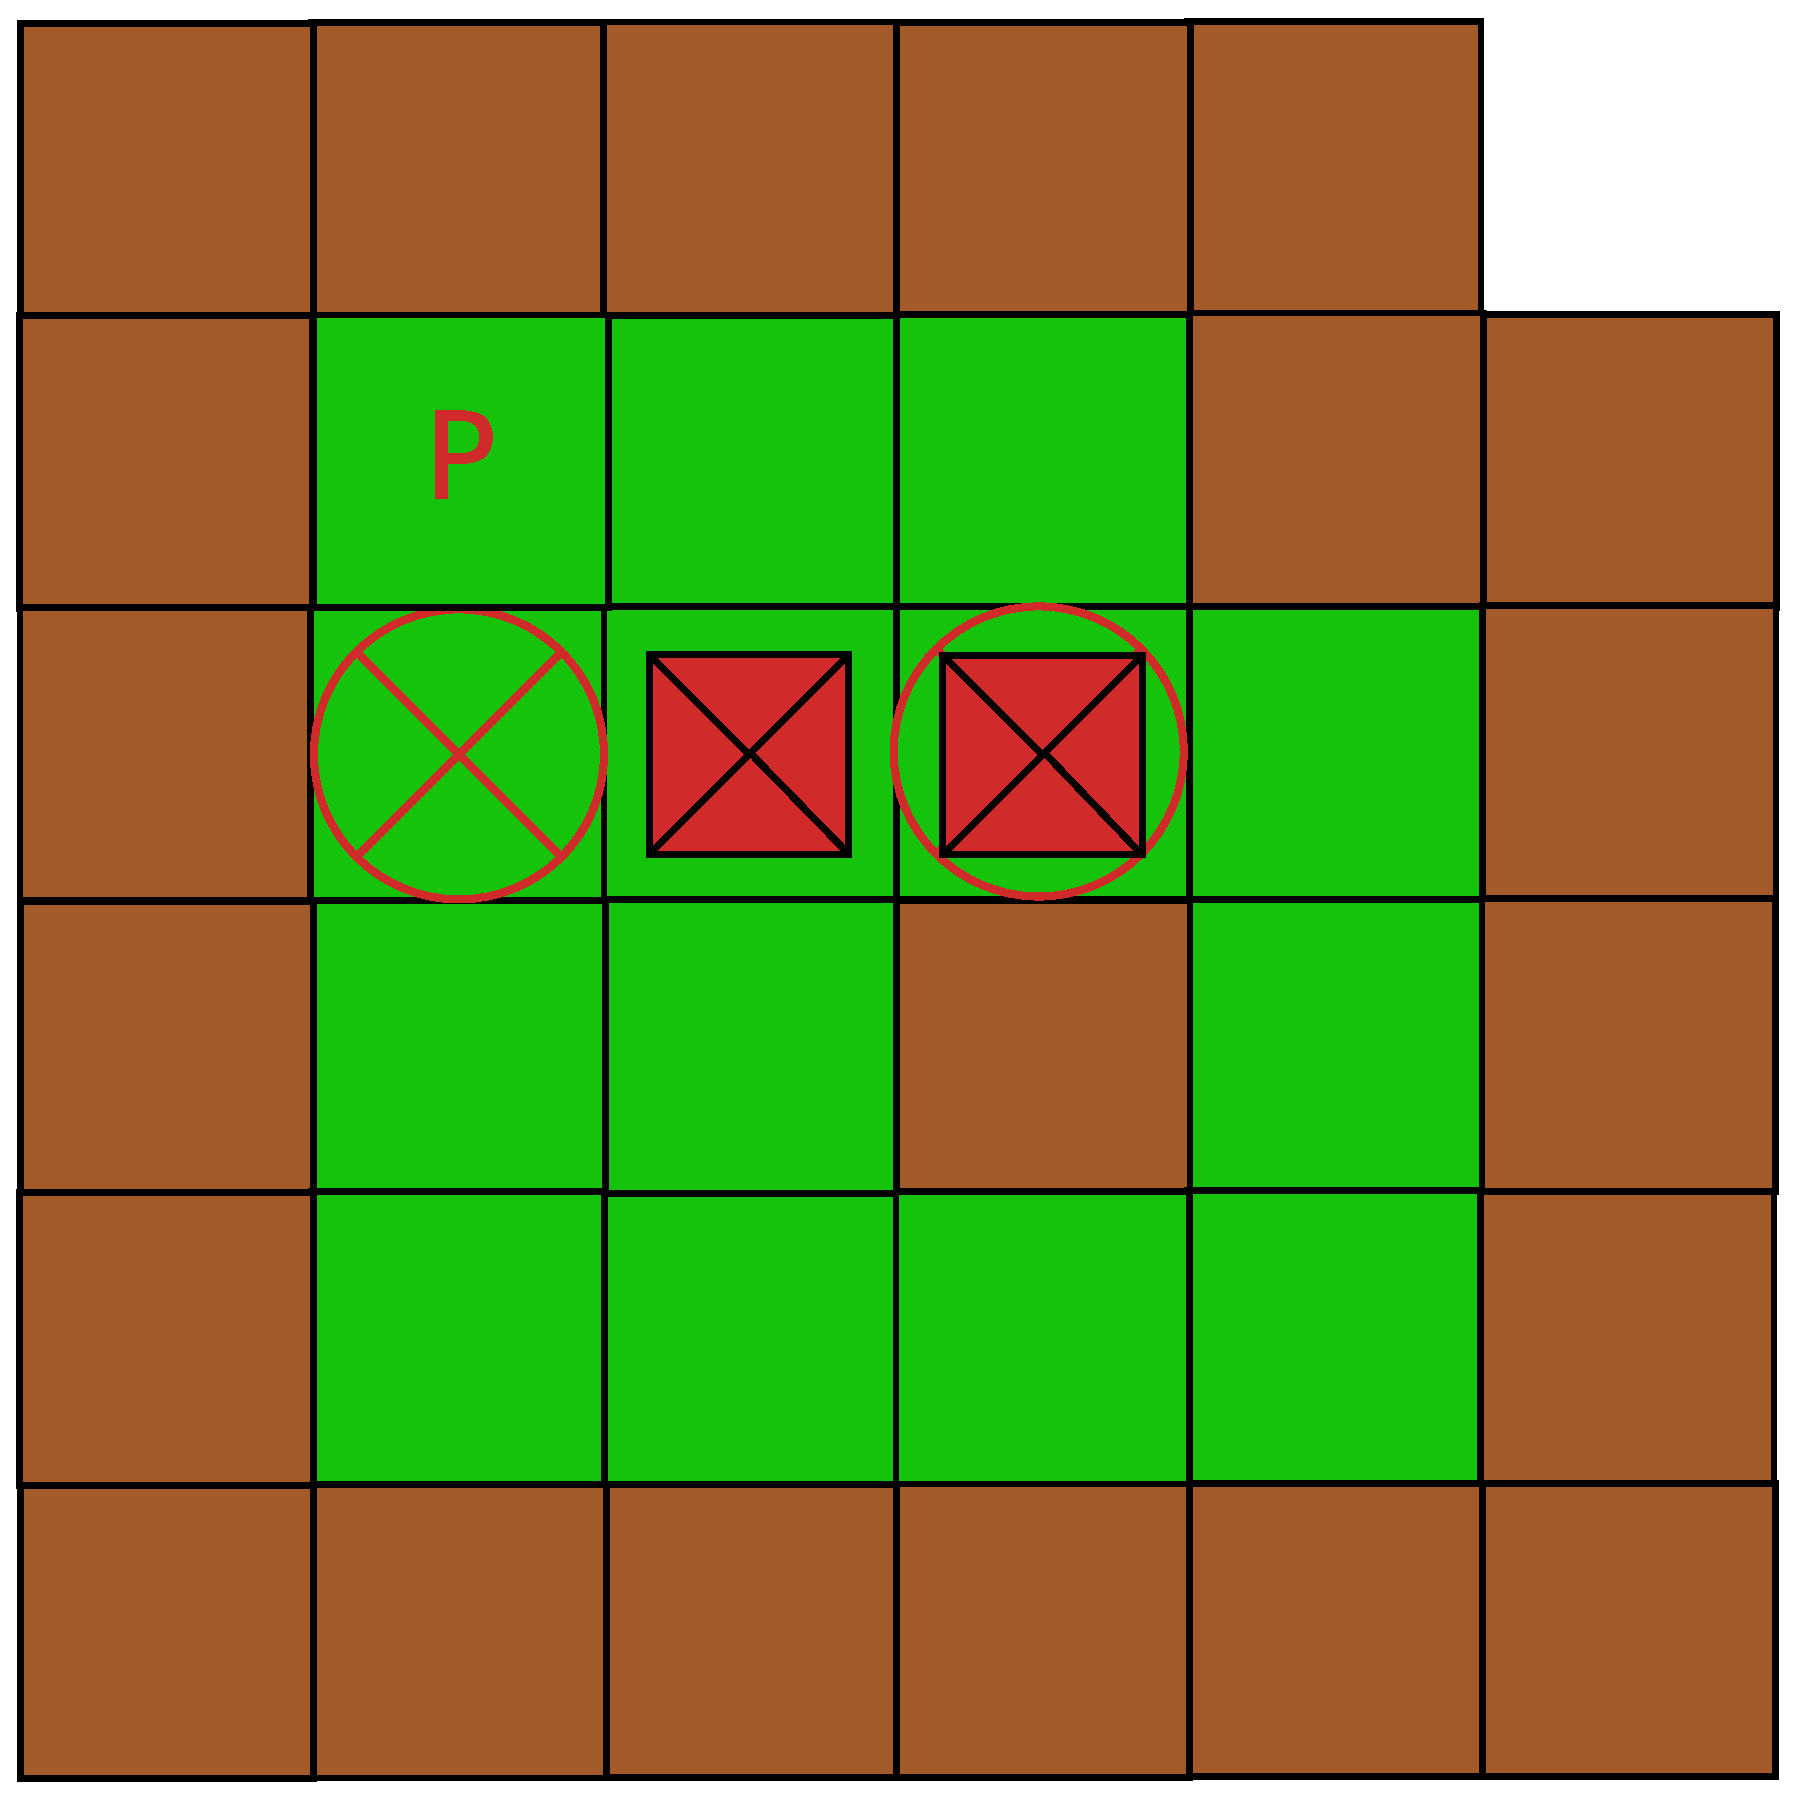
\includegraphics[width=6cm]{Diagram1.eps}
		\caption{Grille de Sokoban. P symbolise le joueur, les ronds rouges sont les cases d'arrivée, et les carrés rouges représentent les caisses.}
		\label{label-figure3}
	\end{figure}
\end{frame}

\begin{frame}{Sokoban - Stratégies de calcul}
	\pause
	Naïf : on considère un coup en tant que déplacement possible du personnage
	\begin{figure}[!h]
		\pause
		\includegraphics[width=3.25cm]{Coup1_strat1.eps}
		\pause
		\includegraphics[width=3.25cm]{Coup2_strat1.eps}
		\pause
		\includegraphics[width=3.25cm]{Coup3_strat1.eps}
	\end{figure}
\end{frame}

\begin{frame}{Sokoban - Stratégies de calcul}
	\pause
	Plus rapide : on ne considère que les coups de déplacement de caisse. On considère alors l'ensemble connexe des cases atteignables depuis celles du personnage
	\begin{figure}[!h]
		\pause
		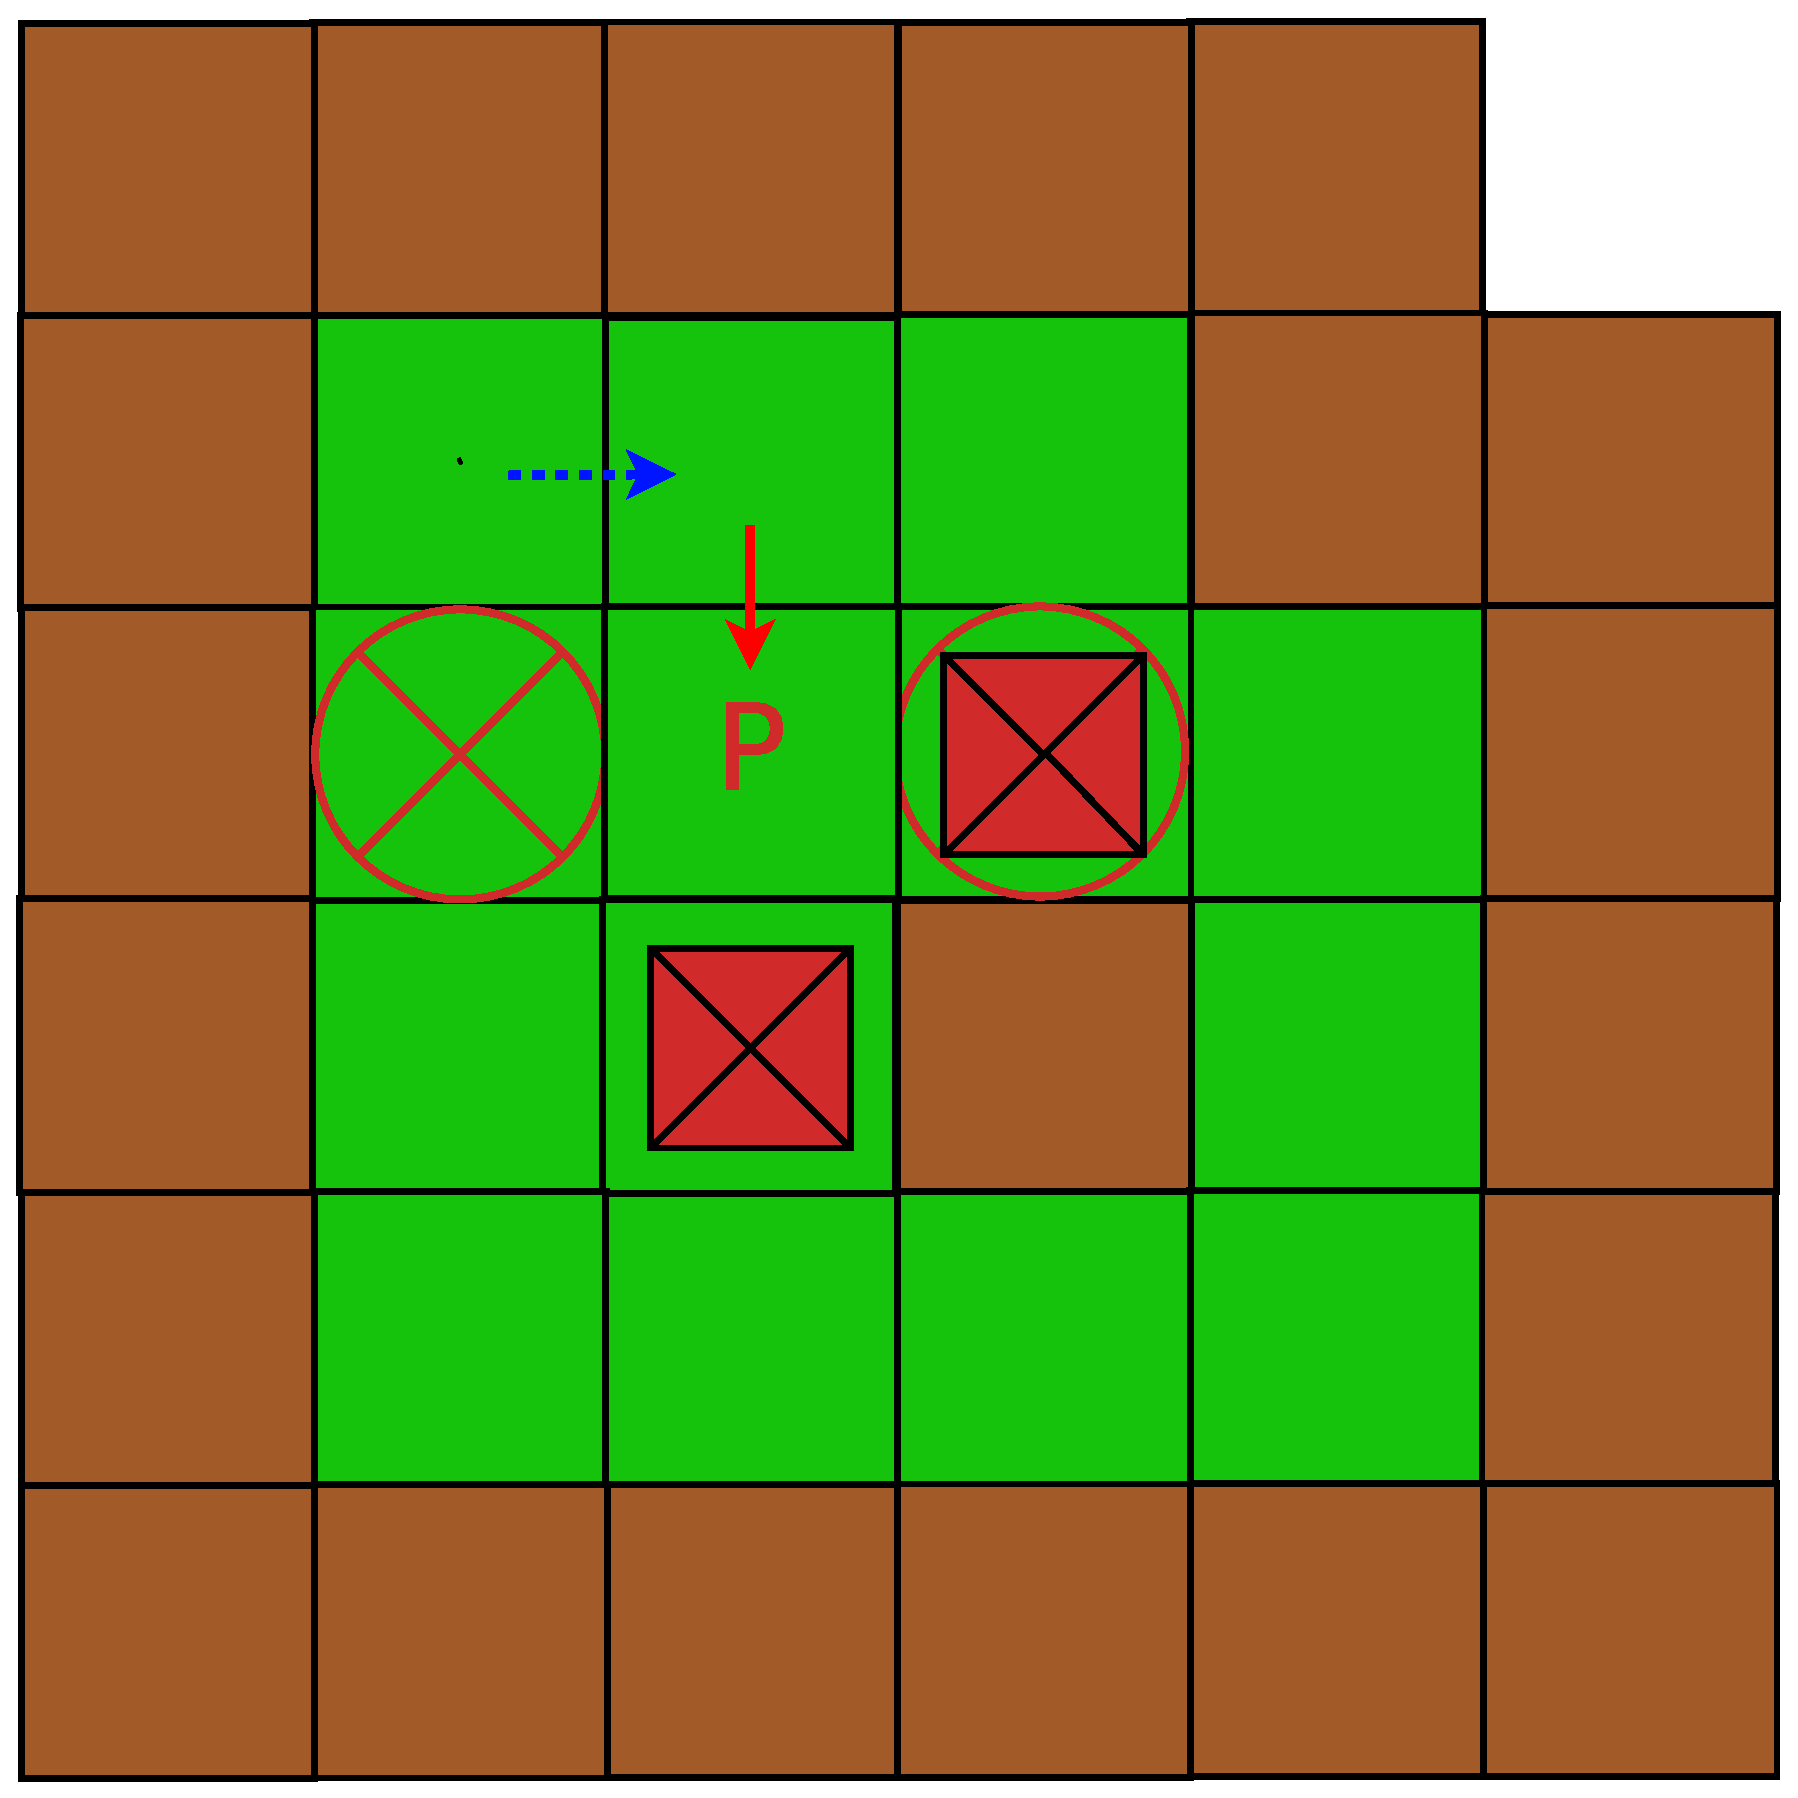
\includegraphics[width=3.25cm]{Coup1_strat2.eps}
		\pause
		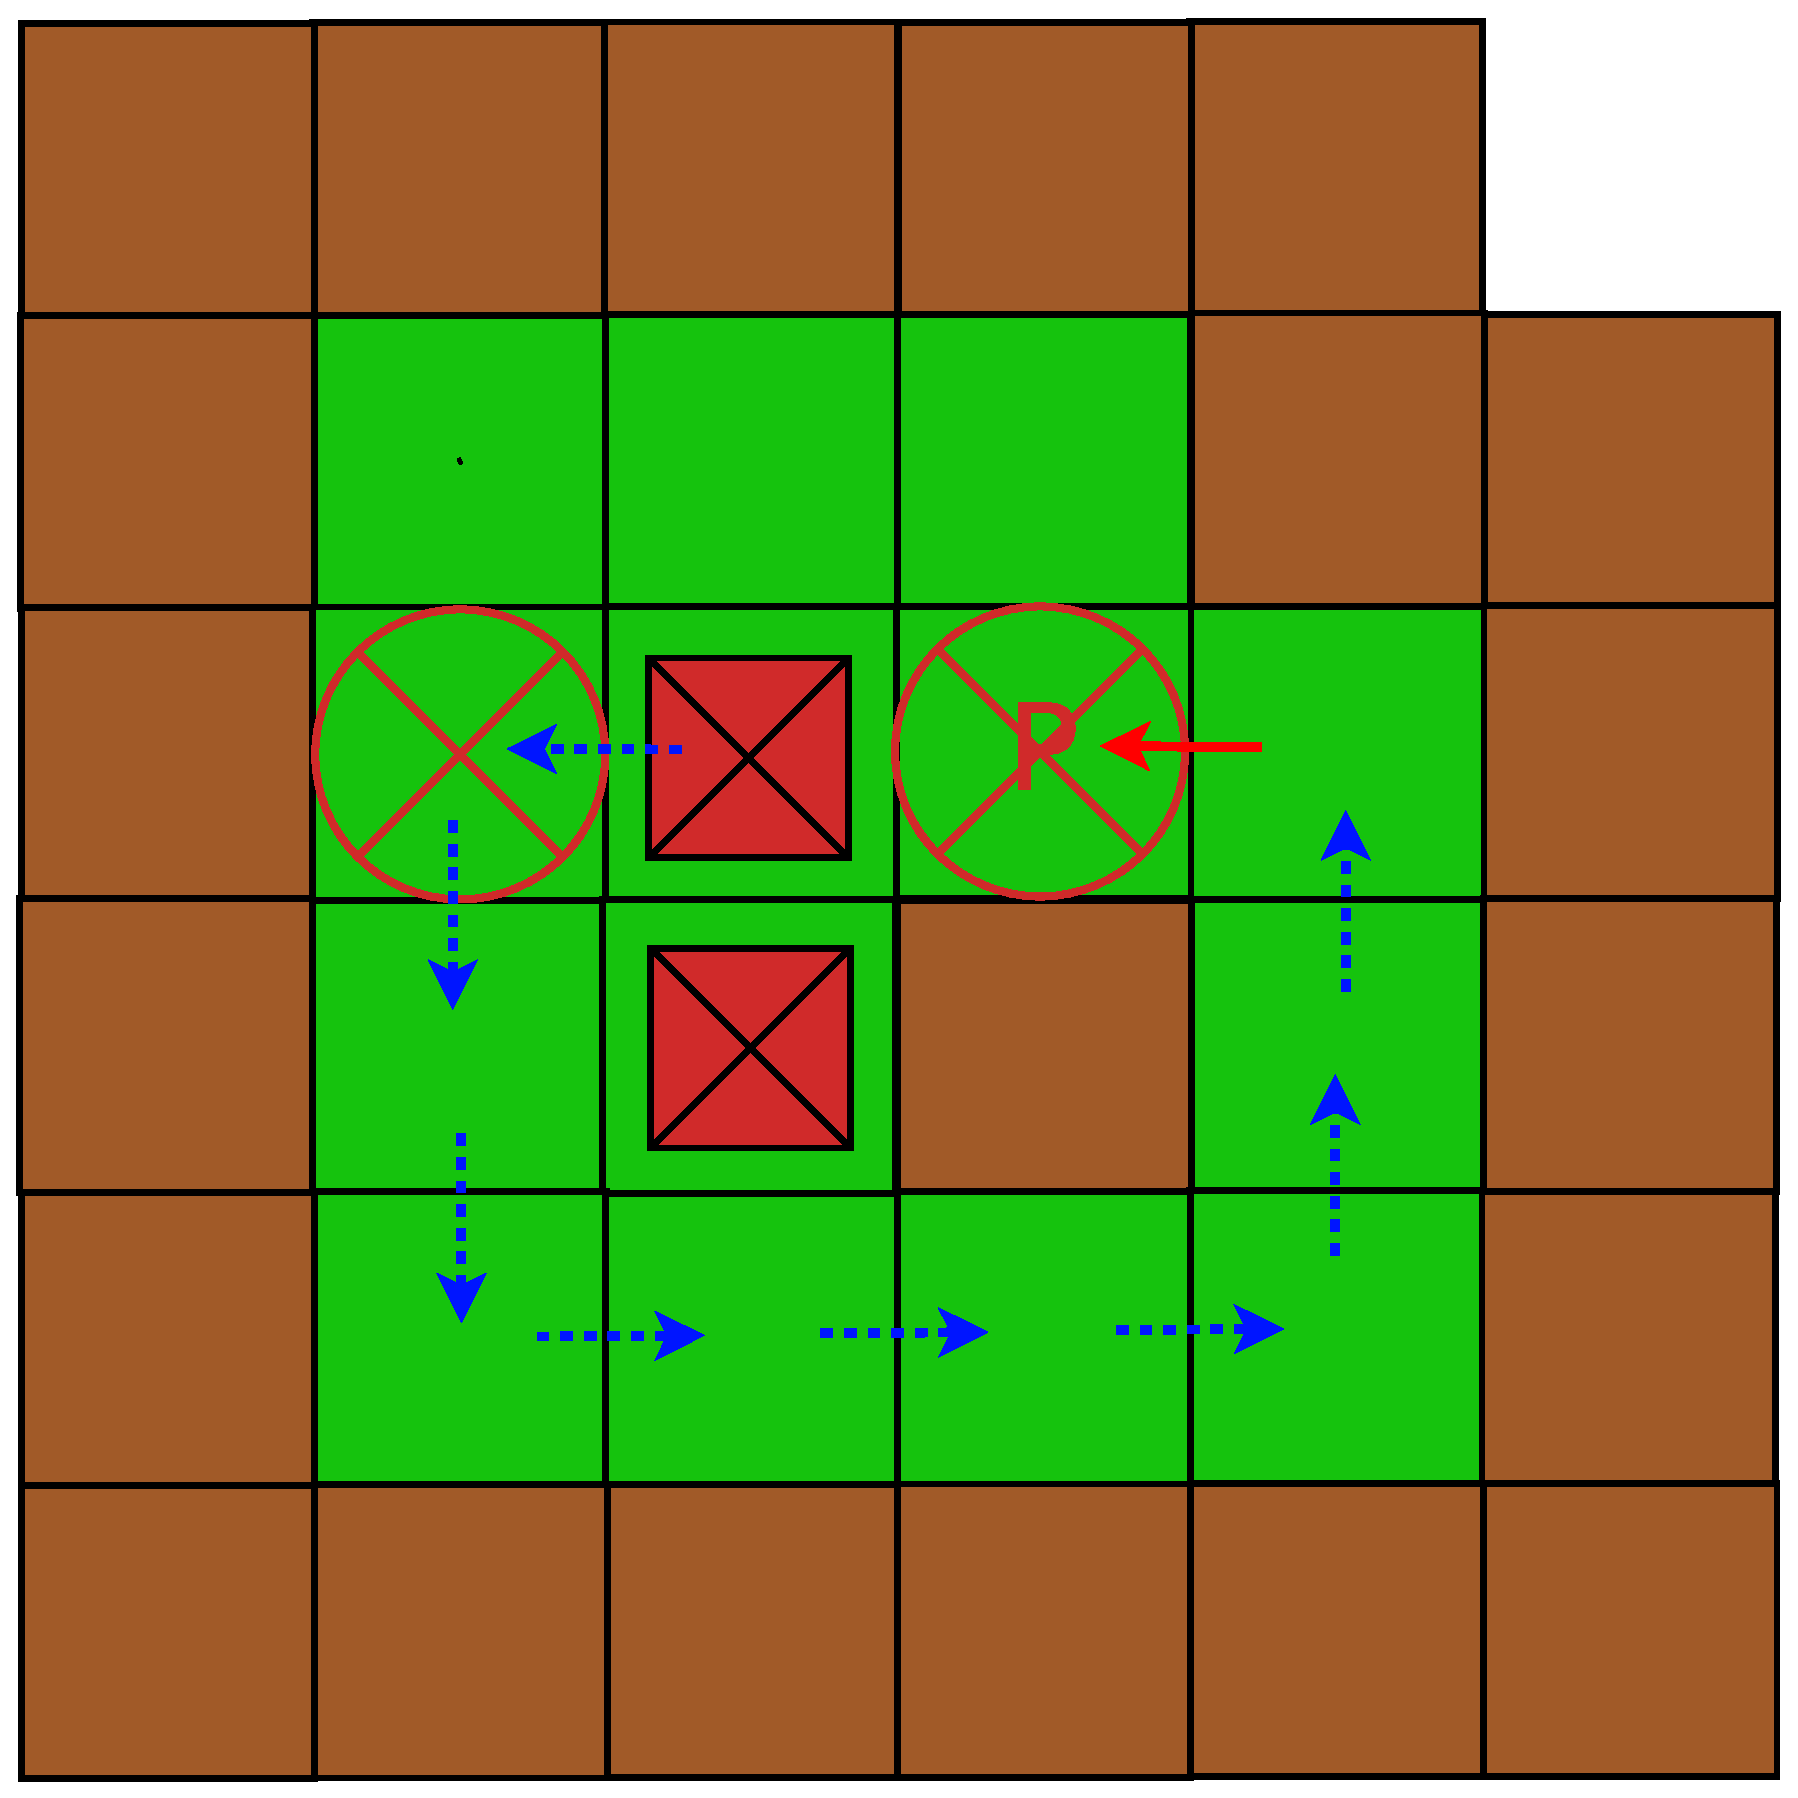
\includegraphics[width=3.25cm]{Coup2_strat2.eps}
		\pause
		\includegraphics[width=3.25cm]{Coup3_strat2.eps}
	\end{figure}
\end{frame}

\begin{frame}{AAN - Schéma}
	\begin{figure}[!h]
		\pause
		\centering  
		\begin{tikzpicture}[apdotsimple/.style={apdot}]
		  \TSort{(0,2)}{a}{3}{r}
		  \TSort{(2.5,0)}{b}{2}{r}
		  \TSort{(5,2)}{c}{3}{r}

		  \path[local transitions]
		    (a_0) edge node[auto] {$b_0$} (a_1)
		    (a_1) edge node[auto] {$b_0$} (a_2)
		    (a_2) edge node[auto] {$b_1$} (a_1)
		    (a_1) edge node[auto] {$b_1$} (a_0)

		    (b_0) edge node[auto] {$c_0$} (b_1)
		    (b_1) edge node[auto] {$a_2$} (b_0)

		    (c_0) edge node[auto] {$b_1$} (c_1)
		    (c_1) edge node[auto] {$b_0$} (c_0)
		    (c_1) edge node[auto] {$a_1$} (c_2)
		    ;
		  \path[local transitions, bend left = 105]
		      (a_0) edge node[auto] {$b_1, c_1$} (a_1)
		    ;
		  \path[local transitions, bend left = 90]
		      (c_0) edge node[auto] {$a_2$} (c_2)
		    ;
		  \path[local transitions, bend left = 90]
		      (c_2) edge node[auto] {$b_1$} (c_0)
		    ;

		  \TState{a_0, b_1, c_1}
		\end{tikzpicture}
		
		\caption{Schéma qui fera office d'exemple de référence}
		\label{label-figure4}
	\end{figure}
\end{frame}

\begin{frame}{AAN - Traduction de l'exemple en ASP}
	En ASP, on définit l'exemple de référence en deux temps.\\
	\begin{itemize}
		\pause
		\item On déclare les niveaux : \\
			\textcolor{blue}{
			automaton\_level("a", 0..2).\\
			automaton\_level("b", 0..1).\\
			automaton\_level("c", 0..2).\\
			}
		\pause
		\item Et les transitions à l'aide de labels : \\
			\textcolor{blue}{
			condition(t1, "a", 0). target(t1, "a", 1). condition(t1, "b", 0).\\
			condition(t2, "a", 1). target(t2, "a", 2). condition(t2, "b", 0).}\\
			\verb![...]!(11 lignes supplémentaires)\\
			\textcolor{blue}{condition(t12, "a", 0). target(t12, "a", 1). condition(t12, "b", 1). condition(t12, "c", 1).\\
			}
	\end{itemize}
\end{frame}

\begin{frame}{Sémantiques}
	\pause
	On s'intéressera à 3 sémantiques : 
	\begin{figure}[!h]
		\pause
		\includegraphics[width=10cm]{Screenshot.png}
		\caption{Schéma repris du pdf Folschette\_Bioss18.pdf de Maxime Folschette}
	\end{figure}
\end{frame}

\begin{frame}{Attracteurs}
	\pause
	Un \textbf{domaine de piège} est un ensemble d'états globaux duquel toutes les transitions globales pour la sémantique choisie mènent à un élément de ce domaine.
	\pause
	Un \textbf{attracteur} est un domaine de piège minimal en terme d'inclusion ensembliste.\\
	\begin{figure}[!h]
		\pause
		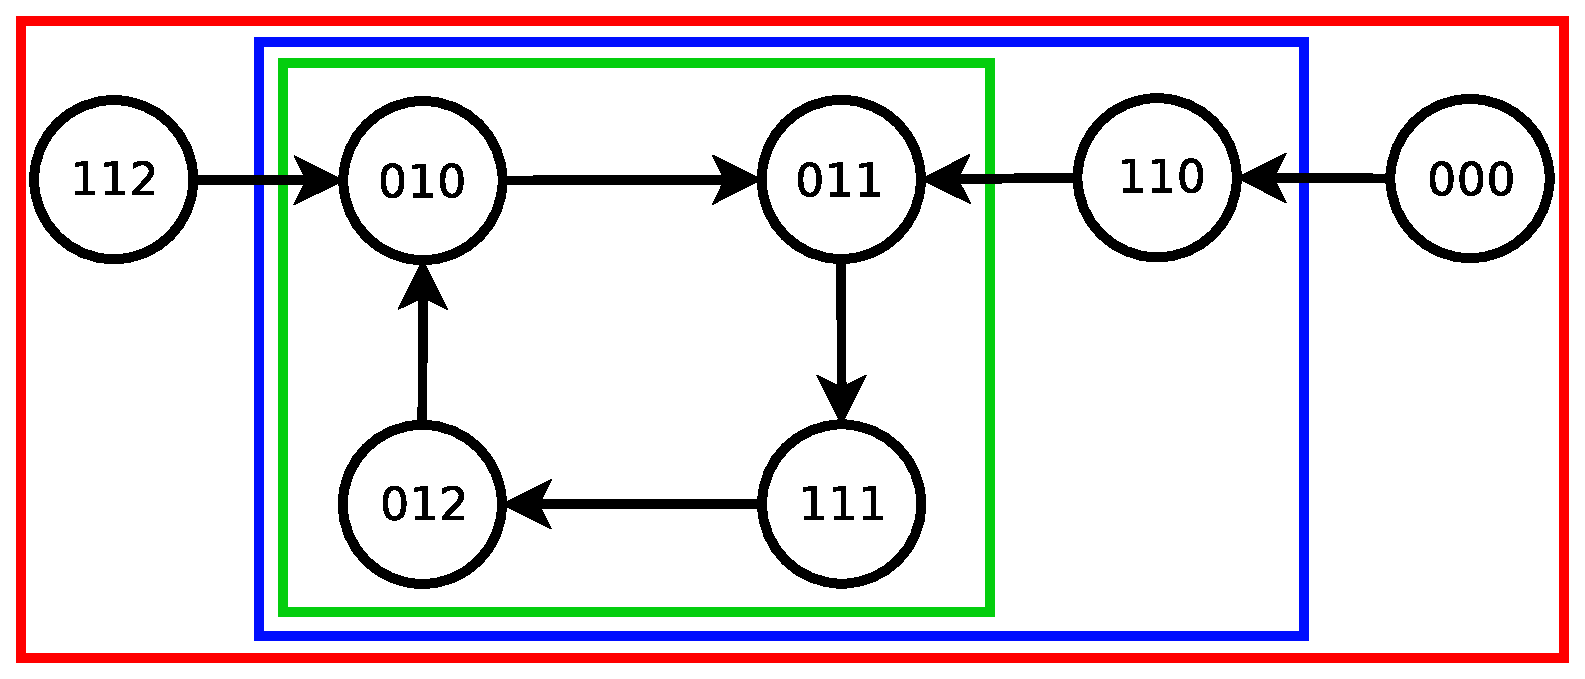
\includegraphics[width=5cm]{presonal_example_synch.eps}
		\includegraphics[width=5cm]{presonal_example_synch2.eps}
		\caption{Sous-graphe du graphe produit de l'exemple de référence avec la sémantique synchrone. \`A gauche, 3 des 6 domaines de piège y sont encadrés. \`A droite, le seul attracteur y est encadré.}
	\end{figure}
	\pause
	\textbf{Lemme :} Les attracteurs d'un AAN sont exactement les domaines de piège cycliques.
\end{frame}

\begin{frame}{Problématique}
	Pour la version synchrone, le code préexistant ne fonctionnait que partiellement : seuls les attracteurs simples (dont les états globaux ont exactement une transition sortante) étaient trouvés.\\
	\begin{figure}[!h]
		\pause
		\begin{tikzpicture}[apdotsimple/.style={apdot}]

			\TSort{(0,2)}{a}{3}{r}
			\TSort{(3,2)}{b}{3}{r}

			\path[local transitions]
			(a_0) edge node[auto] {$b_0$} (a_1)
			(a_1) edge node[auto] {$b_1$} (a_2)
			(a_2) edge node[auto] {$b_1$} (a_1)
			
			(b_0) edge node[auto] {$a_0$} (b_1)
			(b_1) edge node[auto] {$a_1$} (b_2)
			(b_2) edge node[auto] {$a_1$} (b_1)
			;
			
			\path[local transitions, bend left = 90]
			(a_0) edge node[auto] {$b_0$} (a_2)
			;
			
			\path[local transitions, bend left = 90]
			(a_2) edge node[auto] {$b_2$} (a_0)
			;
			
			\path[local transitions, bend left = 90]
			(b_0) edge node[auto] {$a_0$} (b_2)
			;
			
			\path[local transitions, bend left = 90]
			(b_2) edge node[auto] {$a_2$} (b_0)
			;
		\end{tikzpicture}
		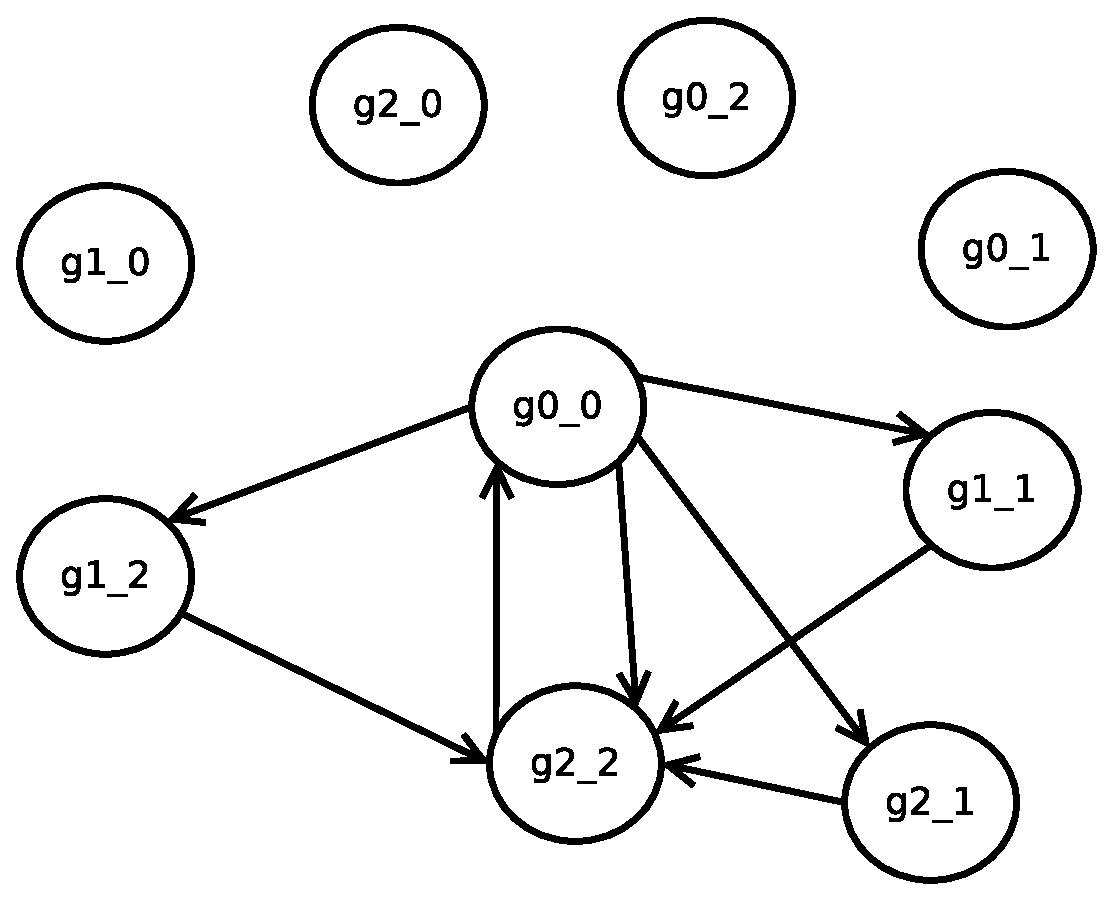
\includegraphics[width=5cm]{Diagram2.eps}
		\caption{Exemple d'AAN sur lequel le code pré-existant ne trouvait pas l'attracteur et graphe produit de celui-ci (pour la sémantique synchrone)}
	\end{figure}
\end{frame}

\begin{frame}{Pistes étudiées}
	\pause
	Solutions étudiées : 
	\begin{itemize}
		\pause
		\item correction de la troisième contrainte en Python
		\pause
		\item utilisation des états globaux en ASP
	\end{itemize}
\end{frame}

\begin{frame}{Correction de la troisième contrainte en Python}
	\pause
	Une fois que l'on a généré tous les chemins possibles dans un AAN à l'aide d'agrégats, il nous faut filtrer les ensembles-solutions qui nous intéressent. On doit alors respecter 3 contraintes : \\
	\begin{itemize}
		\pause
		\item avoir un cycle
		\pause
		\item tous les états globaux du chemin visités après l'étape de fin du visite du cycle doivent être des éléments de ce dernier
		\pause
		\item toutes les transitions globales jouables depuis chacun des éléments du cycle doivent arriver dans un autre élément de ce cycle ( = domaine piège)\\
	\end{itemize}
\end{frame}

\begin{frame}{Correction de la troisième contrainte en Python - Résultats}
	\begin{figure}[!h]
		\begin{tabular}{l|c<{\onslide<2->}c<{\onslide<3->}c<{\onslide<4->}c<{\onslide<5->}c<{\onslide<6->}c<{\onslide<7->}c<{\onslide}c}
			n & exam. & lamb. & trp. & fis. & mamm. & tcr. & t-helper \\ \hline
			$|\Sigma|$ & 4 & 4 & 4 & 9 & 10 & 40 & 101\\ \hline
			2     & 2 & 2 & 0 & 1 & 0 & 0 & 8878+\\
			5     & 2 & 2 & 1 & 1 & 0 & 0 & 5477+\\
			10    & 2 & 2 & 1 & 1 & 1 & 1 & 4072+\\
			15    & 2 & 2 & 1 & 1 & 1 & 1 & 2850+
		\end{tabular}
		\caption{Nombre d'attracteurs trouvés pour la sémantique synchrone (version avec python)}
		\label{label-figure5}
	\end{figure}
	
	\begin{figure}[!h]
		\begin{tabular}{l|c<{\onslide<2->}c<{\onslide<3->}c<{\onslide<4->}c<{\onslide<5->}c<{\onslide<6->}c<{\onslide<7->}c<{\onslide}c}
			n & exam. & lamb. & trp. & fis. & mamm. & tcr. & t-helper \\ \hline
			2     & .051 & .053 & .044 & .047 & .047 & .049 & T.O\\
			5     & .052 & .060 & .039 & .057 & .043 & .079 & T.O\\
			10    & .054 & .076 & .050 & .084 & .082 & .201 & T.O\\
			15    & .093 & .096 & .051 & .108 & .123 & .362 & T.O
		\end{tabular}
		\caption{Temps (en s) de résolution pour la sémantique synchrone (version avec python) - timeout(T.O) = 100s}
		\label{label-figure6}
	\end{figure}
\end{frame}

\begin{frame}{Utilisation des états globaux en ASP}
	\pause
	Une autre manière de gérer la troisième contrainte consiste à créer des prédicats pour les états globaux, et de mémoriser dans la sémantique quels sont les coups jouables depuis un état global, et non une étape temporelle 	
	donnée.\\
	
\end{frame}

\begin{frame}{Seconde solution : travail sur les états globaux - Résultats}
	\begin{figure}[!h]
		\begin{tabular}{l|c<{\onslide<2->}c<{\onslide<3->}c<{\onslide<4->}c<{\onslide<5->}c<{\onslide<6->}c<{\onslide<7->}c<{\onslide}c}
			n & exam. & lamb. & trp. & fis. & mamm. & tcr. & t-helper \\ \hline
			$|\Sigma|$ & 4 & 4 & 4 & 9 & 10 & 40 & 101\\ \hline
			2     & 2 & 2 & 0 &  &  &  & \\
			5     & 2 & 2 & 0 &  &  &  & \\
			10    & 2 &  & 0 &  &  &  & \\
			15    & 2 &  & 1 &  &  &  & 
		\end{tabular}
		\caption{Nombre d'attracteurs trouvés pour la sémantique synchrone (version avec états globaux)}
		\label{label-figure7}
	\end{figure}
	
	\begin{figure}[!h]
		\begin{tabular}{l|c<{\onslide<2->}c<{\onslide<3->}c<{\onslide<4->}c<{\onslide<5->}c<{\onslide<6->}c<{\onslide<7->}c<{\onslide}c}
			n & exam. & lamb. & trp. & fis. & mamm. & tcr. & t-helper \\ \hline
			2     & 3.724 & 43.623 & 4.155 & T.O & T.O & T.O & T.O\\
			5     & 6.457 & 71.786 & 6.288 & T.O & T.O & T.O & T.O\\
			10    & 11.349 & T.O & 11.561 & T.O & T.O & T.O & T.O\\
			15    & 18.767 & T.O & 19.636 & T.O & T.O & T.O & T.O
		\end{tabular}
		\caption{Temps (en s) de résolution pour la sémantique synchrone (version avec états globaux) - timeout(T.O) = 100s}
		\label{label-figure8}
	\end{figure}
\end{frame}

\begin{frame}{Conclusions (et pistes)}
	\begin{itemize}
		\pause
		\item 2 versions fonctionnelles :
		\begin{itemize}
			\item une efficace (en terme de complexité temporelle) avec du filtrage sous Python
			\item l'autre moins efficace avec utilisation d'états globaux (avec quelques fonctions de calcul en Python)
		\end{itemize}
		\pause
		\item Pistes : la seconde version pourrait être améliorée avec de l'incrémental ; considérer des classes d'équivalence des attracteurs, et manipuler des sortes de "bassins d'attraction"
	\end{itemize}
\end{frame}

\begin{frame}{Remerciements}
	Merci à :
	\begin{itemize}
		\item l'ENS de Lyon qui m'a proposé ce stage
		\item Maxime Folschette pour son encadrement
		\item les personnes au sein de l'équipe BioComputing
		\item mes collègues stagiaires de bureau
		\item les auditeurs présents dans cette salle pour leur écoute
	\end{itemize}
\end{frame}

\end{document}



